\documentclass [11pt, a4paper]{article}

\usepackage[slovak]{babel}
\usepackage{times}
\usepackage[utf8]{inputenc}
\usepackage{graphicx}
\usepackage{hyperref}
\usepackage[toc,page]{appendix}
\usepackage[left=2cm, text={17.5cm, 23cm}, top = 2.5cm]{geometry}
\usepackage{siunitx}
\usepackage{pgfplots}

\pgfplotsset{compat=1.12}
\sisetup{
	round-mode          = places,
	round-precision     = 2,
}

\bibliographystyle{czechiso}


\title{Unmasked - Image Inpainting}
\author{Martin Eršek [xersek00], Svätopluk Hanzel [xhanze10]}
\date{\today}


\begin{document}
	\maketitle

	\section{Úvod}
		Image inpainting je metóda, ktorá syntentizuje alternatívny realisticky vyzerajúci vizuálny obraz do vyznačených miest v obrázku tak, aby doplnený obsah vyzeral čo najrealistickejšie a zároveň bol aj sémanticky korektný. Medzi možné využitia tejto metódy patrí napríklad odstránenie nežiadúcich objektov (ľudí alebo predmetov) z obrázku, prípadne takzvaným \uv{retouching}\, nežiadúcich oblastí v obrázku.
	
	\subsection{Existujúce prístupy}
		K riešeniu problému image inpaintingu existuje mnoho navrhovaných prístupov. Tradičné \uv{staré} prístupy za pomoci \uv{patch-based} algoritmov ako \cite{quilting, Efros99}, ktoré progresívne rozširujú pixely blízko okrajov dopĺňanej lokality a na základy nízko úrovňových \uv{features}, akými sú napríklad MSD\footnote{Mean Square Difference} v RGB priestore vyhľadávajú a vkladajú  najpodobnejšie \uv{patches}. Tento starší prístup funguje veľmi dobre na \uv{statických} obrázkoch akými sú napriklad textúry, no má veľké problémy pri \uv{nestatických} obrázkoch.
		Novšie prístupy k image inpaintingu sú založené na hlbokom učení vďaka ktorému je možné priamo predikovať hodnoty dopĺňaných pixelov v inpainting maske. Veľkou výhodou týchto modelov je ich schopnosť naučiť sa adaptívne \uv{features} obrázkov pre rôzne sémantické situácie vyskytujúce sa v obrázkoch. Vďaka tejto vlastnosti sú schopné syntetizovať viac vizuálne uveriteľnejší obsah obzvlášť pre obrázky akými sú napríklad ľudské tváre \cite{li2017generative, yeh2017semantic, globloc, yu2018generative, yu2018free}, objekty \cite{pathak2016context, yu2018free} alebo prírodné scenérie \cite{globloc, yu2018generative, yu2018free}.
	
	\section{Definícia úlohy}
		Rozhodli sme sa implementovať neurónovú sieť, ktorej úlohou bude odstrániť \uv{face-mask}\footnote{Rúško alebo respirátor} z tváre človeka. Úloha pozostáva z detekcie umiestnenia tvárovej masky a 	následnej syntézy pixelov tváre osoby, ktoré sú skryté pod danou maskou tak, aby čo najvierohodnejšie reprezentovali tvár človeka. Keďže je vďaka maske zakrytá tvár skúmanej osoby a o tejto osobe nepoznáme žiadne aditívne informácie, znamená to, že aj keď bude síce doplnená časť tváre vyzerať realisticky, nebude (nemôže) reprezentovať reálnu tvár skúmanej osoby. Túto skutočnosť by bolo možné riešiť doplnením informácií o tvári skúmanej osoby. Týmto spôsobom by bolo možné dopĺňať nie len realisticky vyzerajúce časti tváre pod maskou ale zároveň by toto doplnenie skutočne reprezentovalo tvár skúmanej osoby. Takúto rozšírenú verziu našej úlohy by bolo možné použiť napríklad na \uv{re-touching} rodinných fotiek zo spoločenských oslav na ktorých bolo nosenie tvárových másk povinné. Toto rožšírené zadanie úlohy však ponechávame na prípadné ďalšie práce, ktorých autori by sa rozhodli na našu prácu nadviazať.
	
	\section{Riešenie a implementácia}
		Naše riešenie tohto zadania spočíva primárne v implementácií ML inpainting modelu a jeho natrénovaní na datasete \ref{sec:dataset}.
		
		\subsection{Model}
			Zvolený ML model je GAN sieť - konkrétne SN-PatchGAN \cite{yu2018free}. Od implementácie v pôvodnom článku sme sa odklonili hlavne v tom, že náš model neberie ako vstup 5.-ty, tzv \textit{sketch}, kanál a preto nepodporuje vedené (\textit{guided}) dokreslovanie.
			
			\subsubsection{Gated konvolúcie}\label{sec:gated_conv}
				SN-PatchGAN sa vyznačuje hlavne použitím tzv. \textit{gated} konvolúcií, ktoré nadväzujú na \textit{parciálne konvolúcie}\cite{liu2018image}. Gated konvolúcie na rozdiel od parciálnych konvolúcií umožňujú sieti naučiť sa \textit{soft} masku konvolúcie.
				
				\begin{figure}[h]
					\centering
					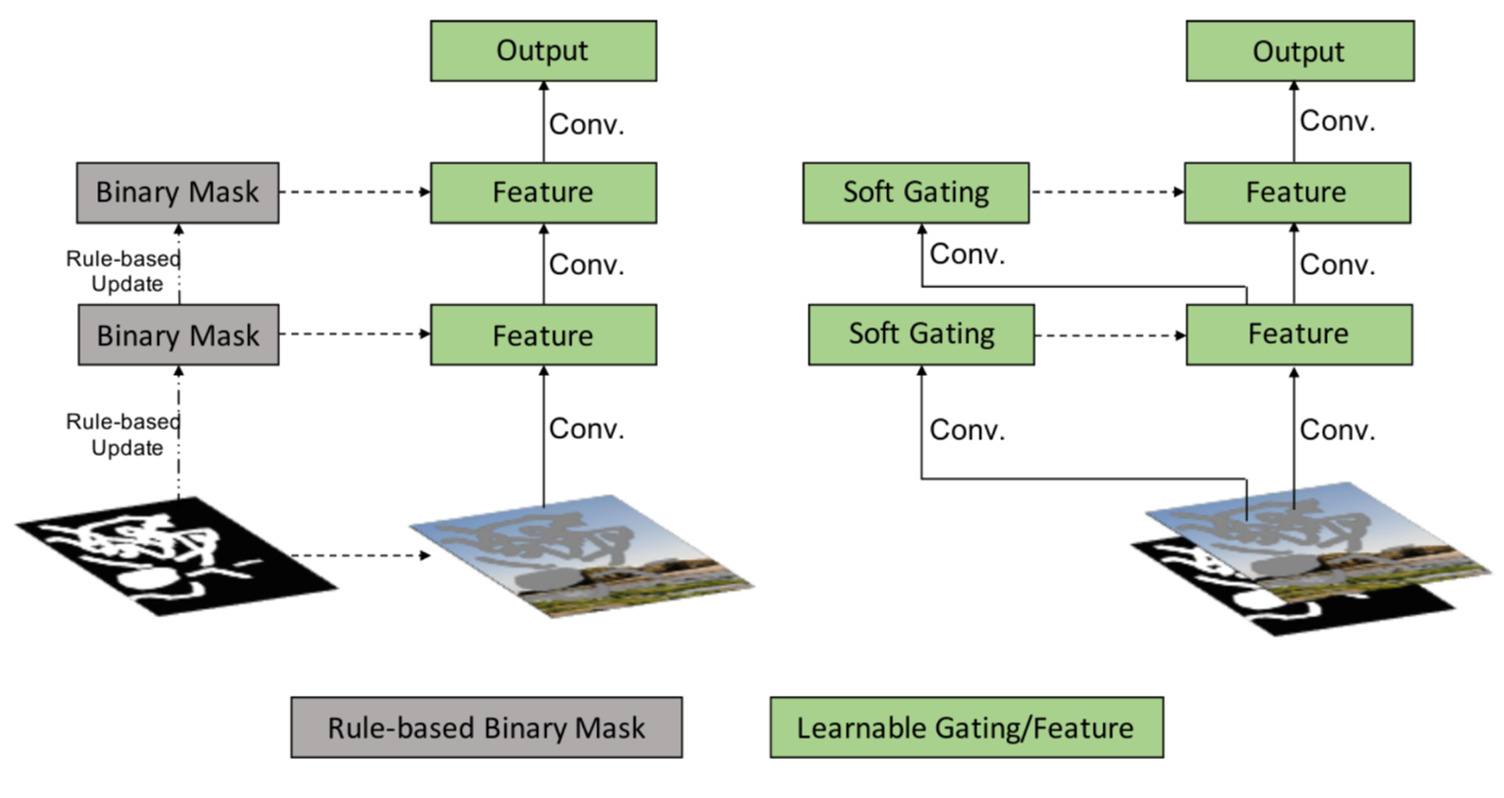
\includegraphics[width=0.7\linewidth]{img/gated-conv}
					\caption{Parciálna vs gated konvolúcia}
					\label{fig:gated-conv}
				\end{figure}
				
			
			\begin{figure}[h]
				\centering
				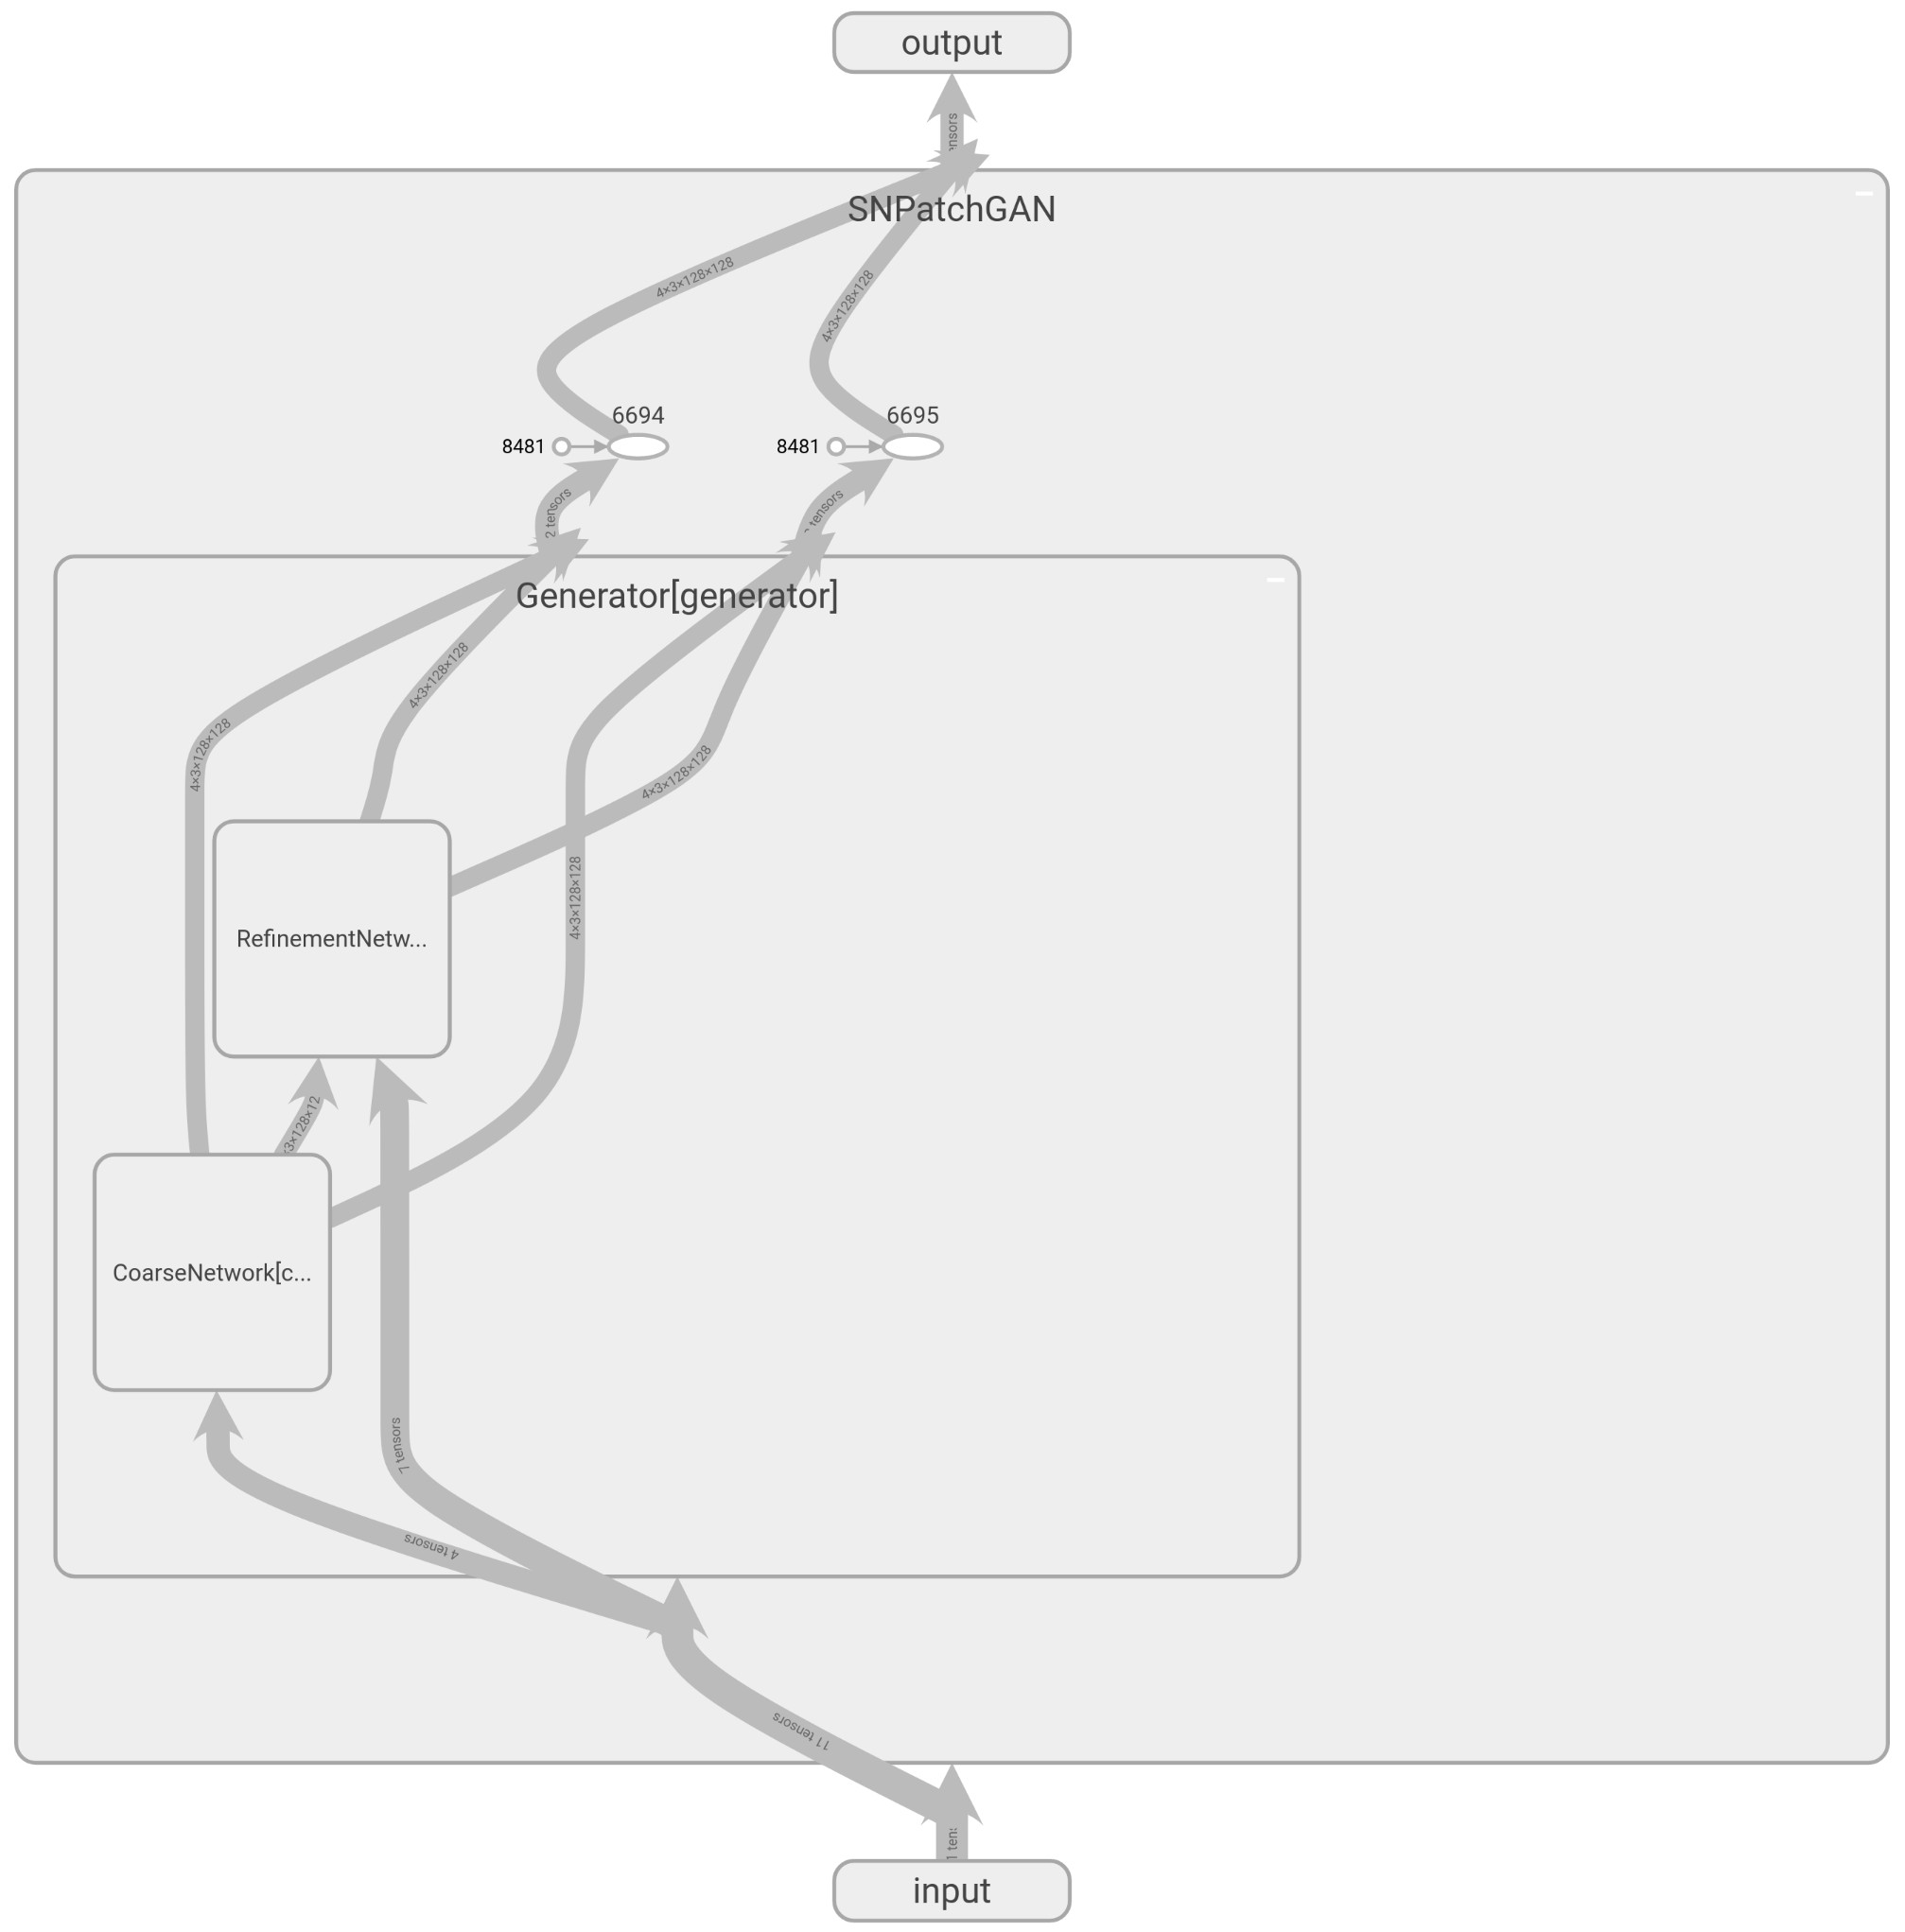
\includegraphics[width=0.8\linewidth]{img/net-arch}
				\caption{Graf siete nášho modelu}
				\label{fig:net-arch}
			\end{figure}
		
			\subsubsection{Generátor}
				Generátor tohto modelu sa skladá z 2 podsietí - \textit{coarse} a \textit{refinement}, pričom prvá z nich má za úlohu vytvoriť priebežný medzivýsledok, zatiaľ čo druhá ho zdokonalí a vykreslí detaily.
				
				Vstupom je 3-kanálový vstupný obrázok a 1-kanálový obrázok - maska, ktorá určuje polohu tvárovej masky vo vstupnom obrázku. Výstupom sú 2 3-kanálové obrázky -- coarse a refined obrázok.
				
				\paragraph{Coarse sieť} sa skladá z niekoľkých konvolučných a dekonvolučných gated\ref{sec:gated_conv} vrstiev, pričom prostredné z nich sú dilatačné.
				\paragraph{Refinement sieť} je mierne komplikovanejšia s dvoma vetvami. Prvá z nich obsahuje \textit{contextual attention} \cite{yu2018generative} vstvu, ktorá sieti umožňuje naučiť sa kedy si má \uv{požičať} informácie z pozadia obrázku. Druhá vetva obsahuje len gated konvolučné vrstvy, pričom niektoré z nich sú dilatačné.
				
			\subsubsection{Diskriminátor}\label{sec:discriminator}
				Diskriminátor je 6-vrstvová plne konvolučná sieť so spektrálnou normalizáciou na všetkých vrstvách. 
				
		\subsection{Implementácia}
			Model je implementovaný v Pythone \footnote{\url{https://www.python.org/}} verzie 3.9 s použitím knižnice PyTorch\footnote{\url{https://pytorch.org/}} a PyTorch Lightning\footnote{\url{https://www.pytorchlightning.ai/}}.
			
			\paragraph{PyTorch Lightning} je pomocná knižnica PyTorch, ktorá zjednodušuje prácu s PyTorch a umožnuje spúšťanie kódu na rôznych platformách bez potreby zmeny kódu. Vďaka tomu môžeme náš kód spustiť na CPU, CUDA GPU aj TPU bez zmeny kódu. Zároveň podporuje aj distribuované učenie na viacerých grafických kartách, čo nám veľmi zrýchlilo trénovanie a pomohlo s experimentami.
			
			Samotná implementácia siete je realizovaná v moduli \texttt{network}, pričom PyTorch modul obaľujúci celú sieť je implementovaný cez triedu \texttt{SNPatchGAN} v súbore \texttt{gan.py}. Všetky ostatné podsiete, rovnako ako vrstvy sú uložené v samostatných súboroch pre lepšiu orientáciu a udržateľnosť kódu.
				
		
		\subsection{Dataset}\label{sec:dataset}
			Pre trénovanie tohto modelu sme použili dataset CelebA-HQ \cite{liu2015faceattributes}, ktorý obsahuje celkovo 30 000 obrázkov tvárí celebrít v rozlíšení 1024x1024px. Tieto fotky sú však bez prekrytia tváre, ktoré potrebujeme pre tento projekt.
			
			Pre potreby trénovania siete sme vytvorili triedu \texttt{MaskedCelebADataset}\footnote{súbor \texttt{dataset.py}}, ktorá dokáže načitavať obrázky z určeného miesta, aplikovať na ne on-the-fly masku a vrátiť tieto dáta vo formáte vhodnom pre ďalšie spracovanie sieťou. Táto trieda očakáva cestu k zložke s datasetom, pričom táto zložka ďalej musí obsahovať zložku \texttt{images}, v ktorej sú priamo umiestnené všetky obrázky.
			
			\paragraph{Rozdelenie dát} Dataset obsahuje 30 000 obrázkov, ktoré sme rozdelili v pomere 70:30 na trénovacie a validačné vzorky, takže validácia prebiehala vždy len na obrázkoch, ktoré táto sieť ešte nevidela.
			
			\subsubsection{Maskovanie tváre}
				Na prekrytie tváre sme použili projekt MaskTheFace\footnote{\url{https://github.com/aqeelanwar/MaskTheFace}} \cite{anwar2020masked}, ktorý dokáže pomocou predučeného modelu rozoznať rysy tváre a podľa nich vložiť jeden z preddefinovaných obrázkov masiek na správne miesto spolu s natočením a zmenou veľkosti masky, čím sa zvyšuje dôveryhodnosť výsledku.
				
				\begin{figure}[h]
					\centering
					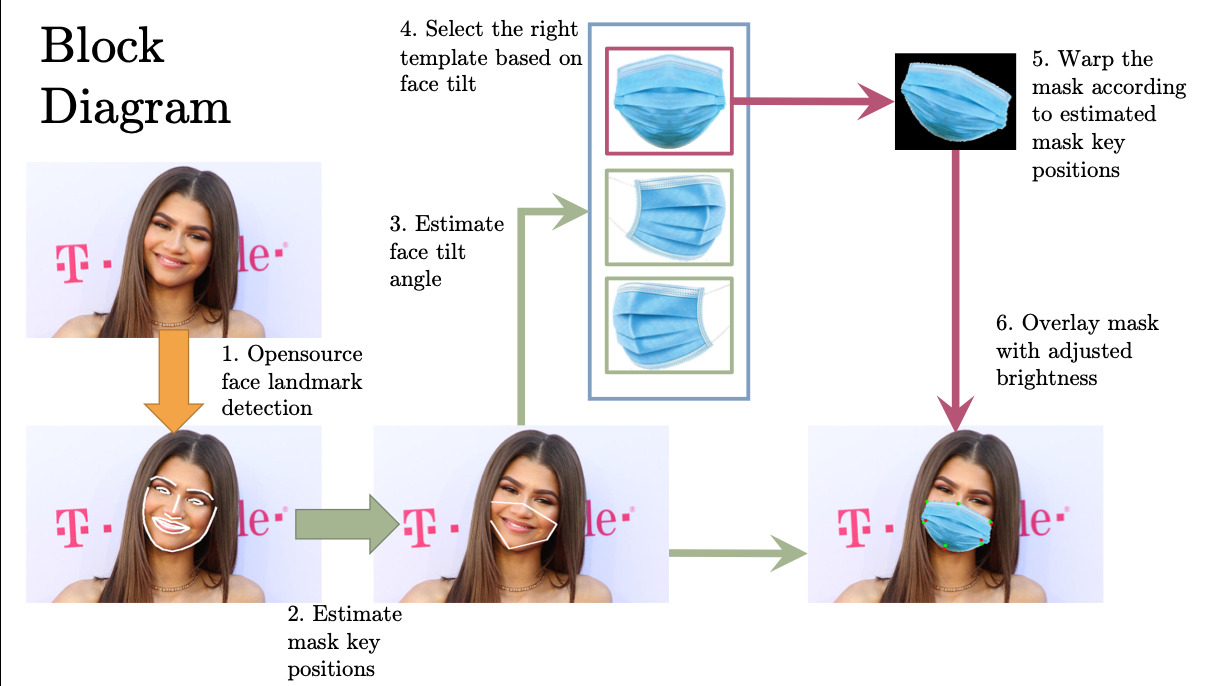
\includegraphics[width=0.7\linewidth]{img/mask_the_face-diagram}
					\caption{Diagram fungovania maskovania tváre \cite{anwar2020masked}}
					\label{fig:masktheface-diagram}
				\end{figure}
				
				V rámci riešenia projektu UnMasked sme zároveň refaktorovali MaskTheFace, prerobili sme ho na importovateľnú python knižnicu a zjednodušili niektoré volania v ňom. Tieto zmeny nám umožnili vytvorenie on-the-fly maskovania počas trénovania. Zároveň sa chystáme doplniť funkcionalitu, ktorá pre nás nebola potrebná a vytvoriť merge request z nášho\footnote{\url{https://github.com/sveatlo/MaskTheFace/}} do pôvodného repozitára.
			
		\subsection{Trénovanie}
			Trénovanie siete prebiehalo na 1 počítači s dvomi grafikami - NVIDIA GTX1080 8GB a NVIDIA GTX1070 8GB.
			
			Trénovací skript je implementovaný v \texttt{train.py} a umožňuje predávanie hyperparametrov siete cez jednoduché používateľské rozhranie. Najdôležitejšími parametrami sú:
			\begin{itemize}
				\item \texttt{--gpus}, ktorý umožňuje zvoliť počet GPU, ktoré sa majú použiť
				\item \texttt{--resume\_checkpoint}, ktorý umožňuje obnoviť prerušené trénovanie
			\end{itemize}
		
			\paragraph{Batch size} je voliteľná pomocou prepínača \texttt{--batch\_size}, pričom nám sa počas testovania s obrázkami veľkosti 256x256px najviac osvedčila veľkosť 16.
			\paragraph{Optimalizátor} Pre učenie generátora aj diskriminátora je použitý stochastický optimalizátor Adam \cite{kingma2017adam}. Rozdiel medzi optimalizáciou generátora a diskriminátora je, že optimilizátor pre diskriminátor sa spúšťa len raz za 5 batch-ov, čo zabraňuje jeho rýchlemu preučeniu.
			\paragraph{Loss funkcia} Celková loss funkcia pre generátor je výsledkom spojenia L1 loss funkcie na coarse a refined obrázkoch, lokálnej loss funkcie (výstup diskriminátora \ref{sec:discriminator}) a globálnej loss funkcie (výstup perceptual network - predučená sieť VGG16).
			\paragraph{Learning rate} je nastaviteľná samostatne pre generátor a diskriminátor. Nám sa overila hodnota 2e-4, vďaka ktorej sme dosiahli stabilné učenie.
			
			\begin{figure}[h]
				\centering
				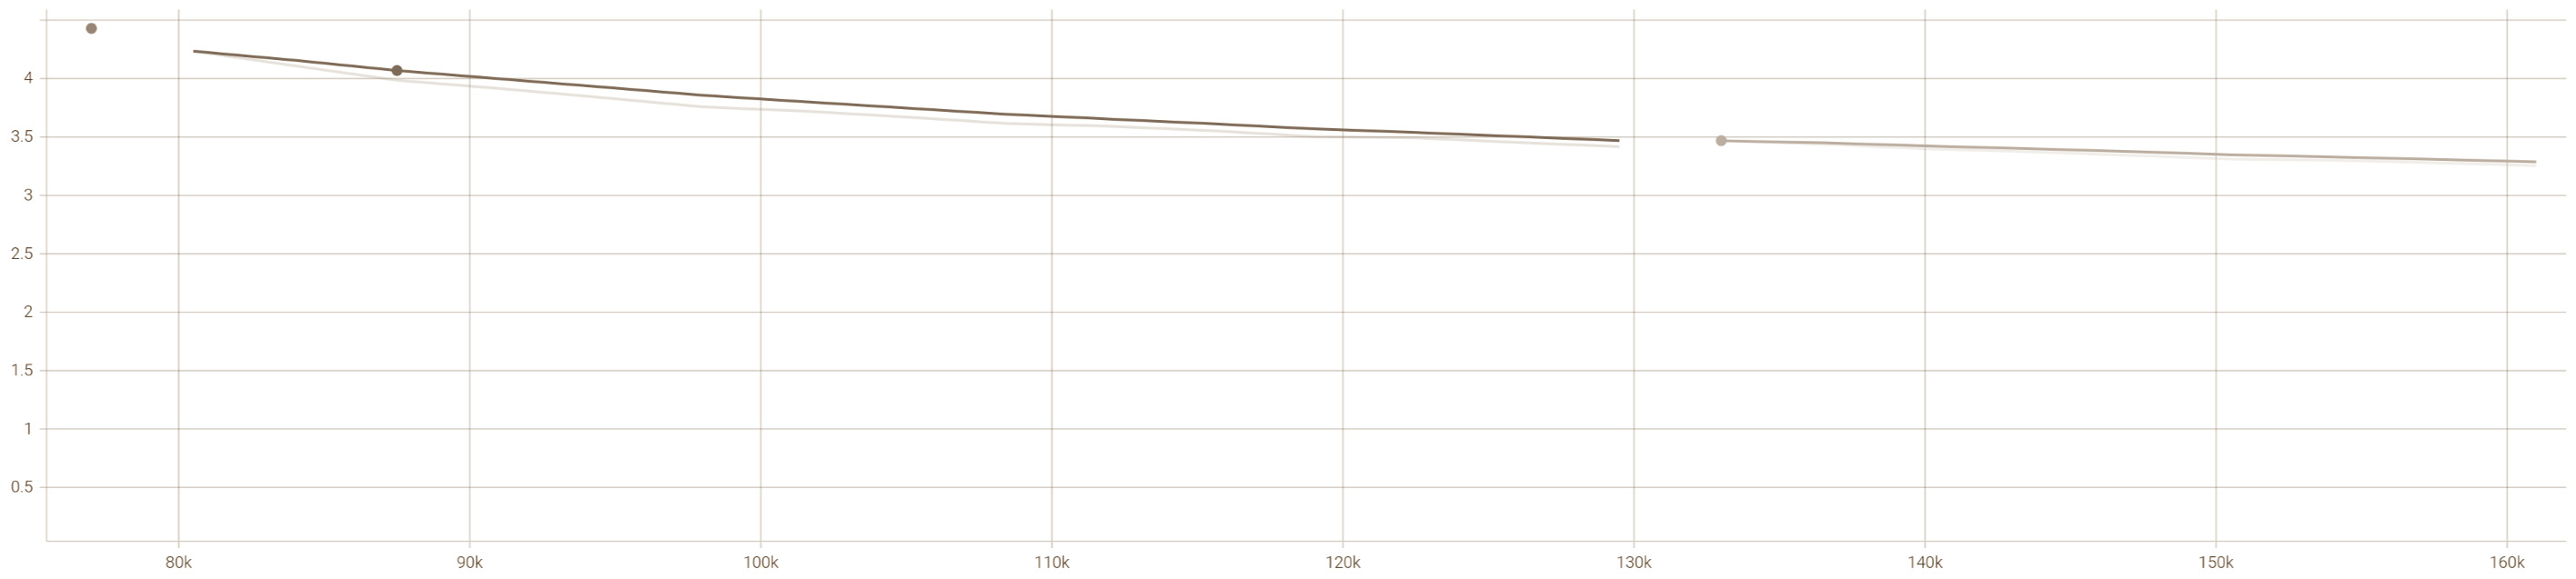
\includegraphics[width=1\linewidth]{img/validation-perceptual-loss-progress}
				\caption{Priebeh perceptual loss}
				\label{fig:validation-perceptual-loss-progress}
			\end{figure}
			
		
	\section{Vyhodnotenie}
		Vyhodnotenie nášho modelu sme vykonali za pomoci užívateľského výskumu, ktoré sa zúčastnilo 10 užívateľov. Ich úlohou bolo ohodnotiť rôzne výstupné obrázky modelu a určiť na škále od 1 do 10 ako veľmi realistický je výstup nášho modelu. Skóre 10 značí, že si užívateľ myslí, že obrázok vyzerá ako reálny obrázok (fotografia) a nebol nijako upravovaný počítačom. Skóre 1 značí, že je zjavné, že obrázok nie je reálny a do obrázku niečo dokresloval počítač. Užívatelia hodnotili subjektívne a to tak, že pokiaľ tvár vyzerala uveriteľne no obsahovala nejaký miniatúrny artefakt, ktorý spozorovali až po dlhšom skúmaní, tak uviedli skóre blížiace sa viac k 10. V opačnom prípade sa blížili k 1. Skóre jedna udeľovali naozaj len v prípadoch pokiaľ doplnená časť tváre do obrázku absolutne nesedela. Ako možno vidieť z obrázku \ref{user_research}, veľké množstvo výstupných fotografií dostalo skóre 10 značiace, že užívatelia by nevedeli rozpoznať či sa jedná o skutočnú fotografiu alebo počítač tak dokonale dokreslil úsek tváre, že to nie je možné rozoznať. Tento poznatok značí, že náš model funguje úspešne tak ako má.
		
		\begin{figure}[h!]
			\begin{center}
				\begin{tikzpicture}
					\begin{axis}[
						width=0.9\linewidth, height=8cm,
						grid=major,
						grid style={dashed,gray!30},
						xlabel=Skóre,
						ylabel=Počet hodnotení týmto skóre,
						legend style={at={(0.5,-0.2)},anchor=north},
						xtick=data,
						ybar,
						]
						\addplot[blue, fill] table[x=score,y=count, col sep=comma] {user_research_male_csv};
						\addlegendentry{male}
						\addplot[red, fill] table[x=score,y=count, col sep=comma] {user_research_female_csv};
						\addlegendentry{female}
					\end{axis}
				\end{tikzpicture}
				\caption{Ohodnotenie vierohodnosti obrázka za pomoci užívateľského výskumu. X-ová os značí to ako veľmi realisticky vyzeral obrázok pre užívateľov. 1 - nerealistický, generovaný počítačom; 10 - originálna neupravovaná fotka.}
				\label{user_research}
			\end{center}
		\end{figure}
		
		Nižšie skóre dostali prevažne obrázky obsahujúce tvár celebrity v netypickej polohe, prípadne pokiaľ bola tvár celebrity niečím čiastočne prekrytá - napríklad rukou alebo palicou\footnote{V datasete existovali aj obrázky kde celebrita držala v ruke palicu, ktorá prekrývala časť jej tváre.}.
		
		
	
	\newpage
	\renewcommand{\refname}{Zdroje}
	\bibliography{references}
	
	
	\begin{appendices}
		\section{Ukážka výstupov z modelu}
		todo
	\end{appendices}

\end{document}
